\chapter{Figuras complementares da explicabilidade}
\label{ap:figuras}

Este apêndice traz as figuras da trilha de proporção de alfabetizados, que
acompanham as da trilha de proficiência apresentadas na
Seção~\ref{sec:res-xai}. Na trilha de proporção, o SHAP está na escala da
margem do modelo (log-odds), e o LIME, na da proporção prevista.

\begin{figure}[H]
    \centering
    \caption{Contribuições SHAP das 12 variáveis principais na trilha de proporção de alfabetizados}
    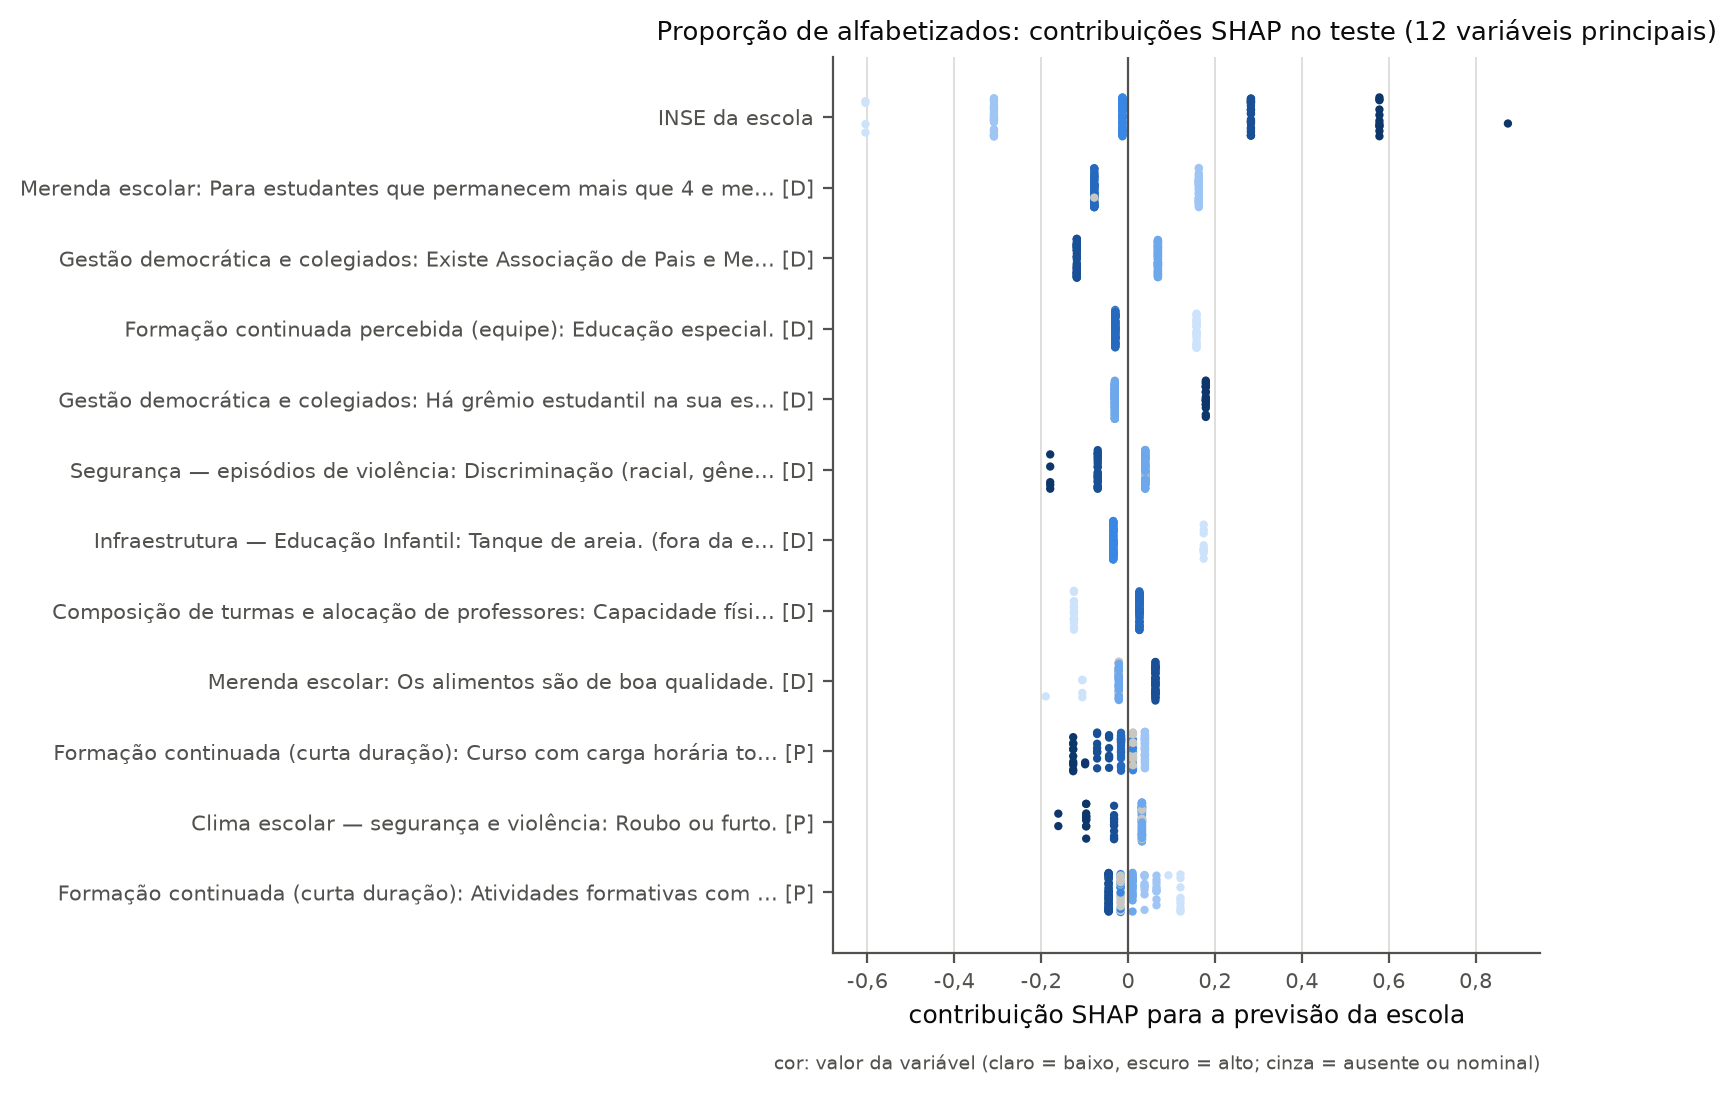
\includegraphics[width=\textwidth]{figuras/shap_resumo_prop.png}
    \begin{flushleft}
    {\footnotesize Fonte: elaborada pelo autor, com base nos microdados do
    Saeb 2023 (Inep). Cada ponto é uma escola do conjunto de teste. [P]:
    questionário do professor. [D]: questionário do diretor.}
    \end{flushleft}
    \label{fig:ap-shap-prop}
\end{figure}

\begin{figure}[H]
    \centering
    \caption{Participação com sinal das variáveis no SHAP e no LIME nas três escolas da trilha de proporção}
    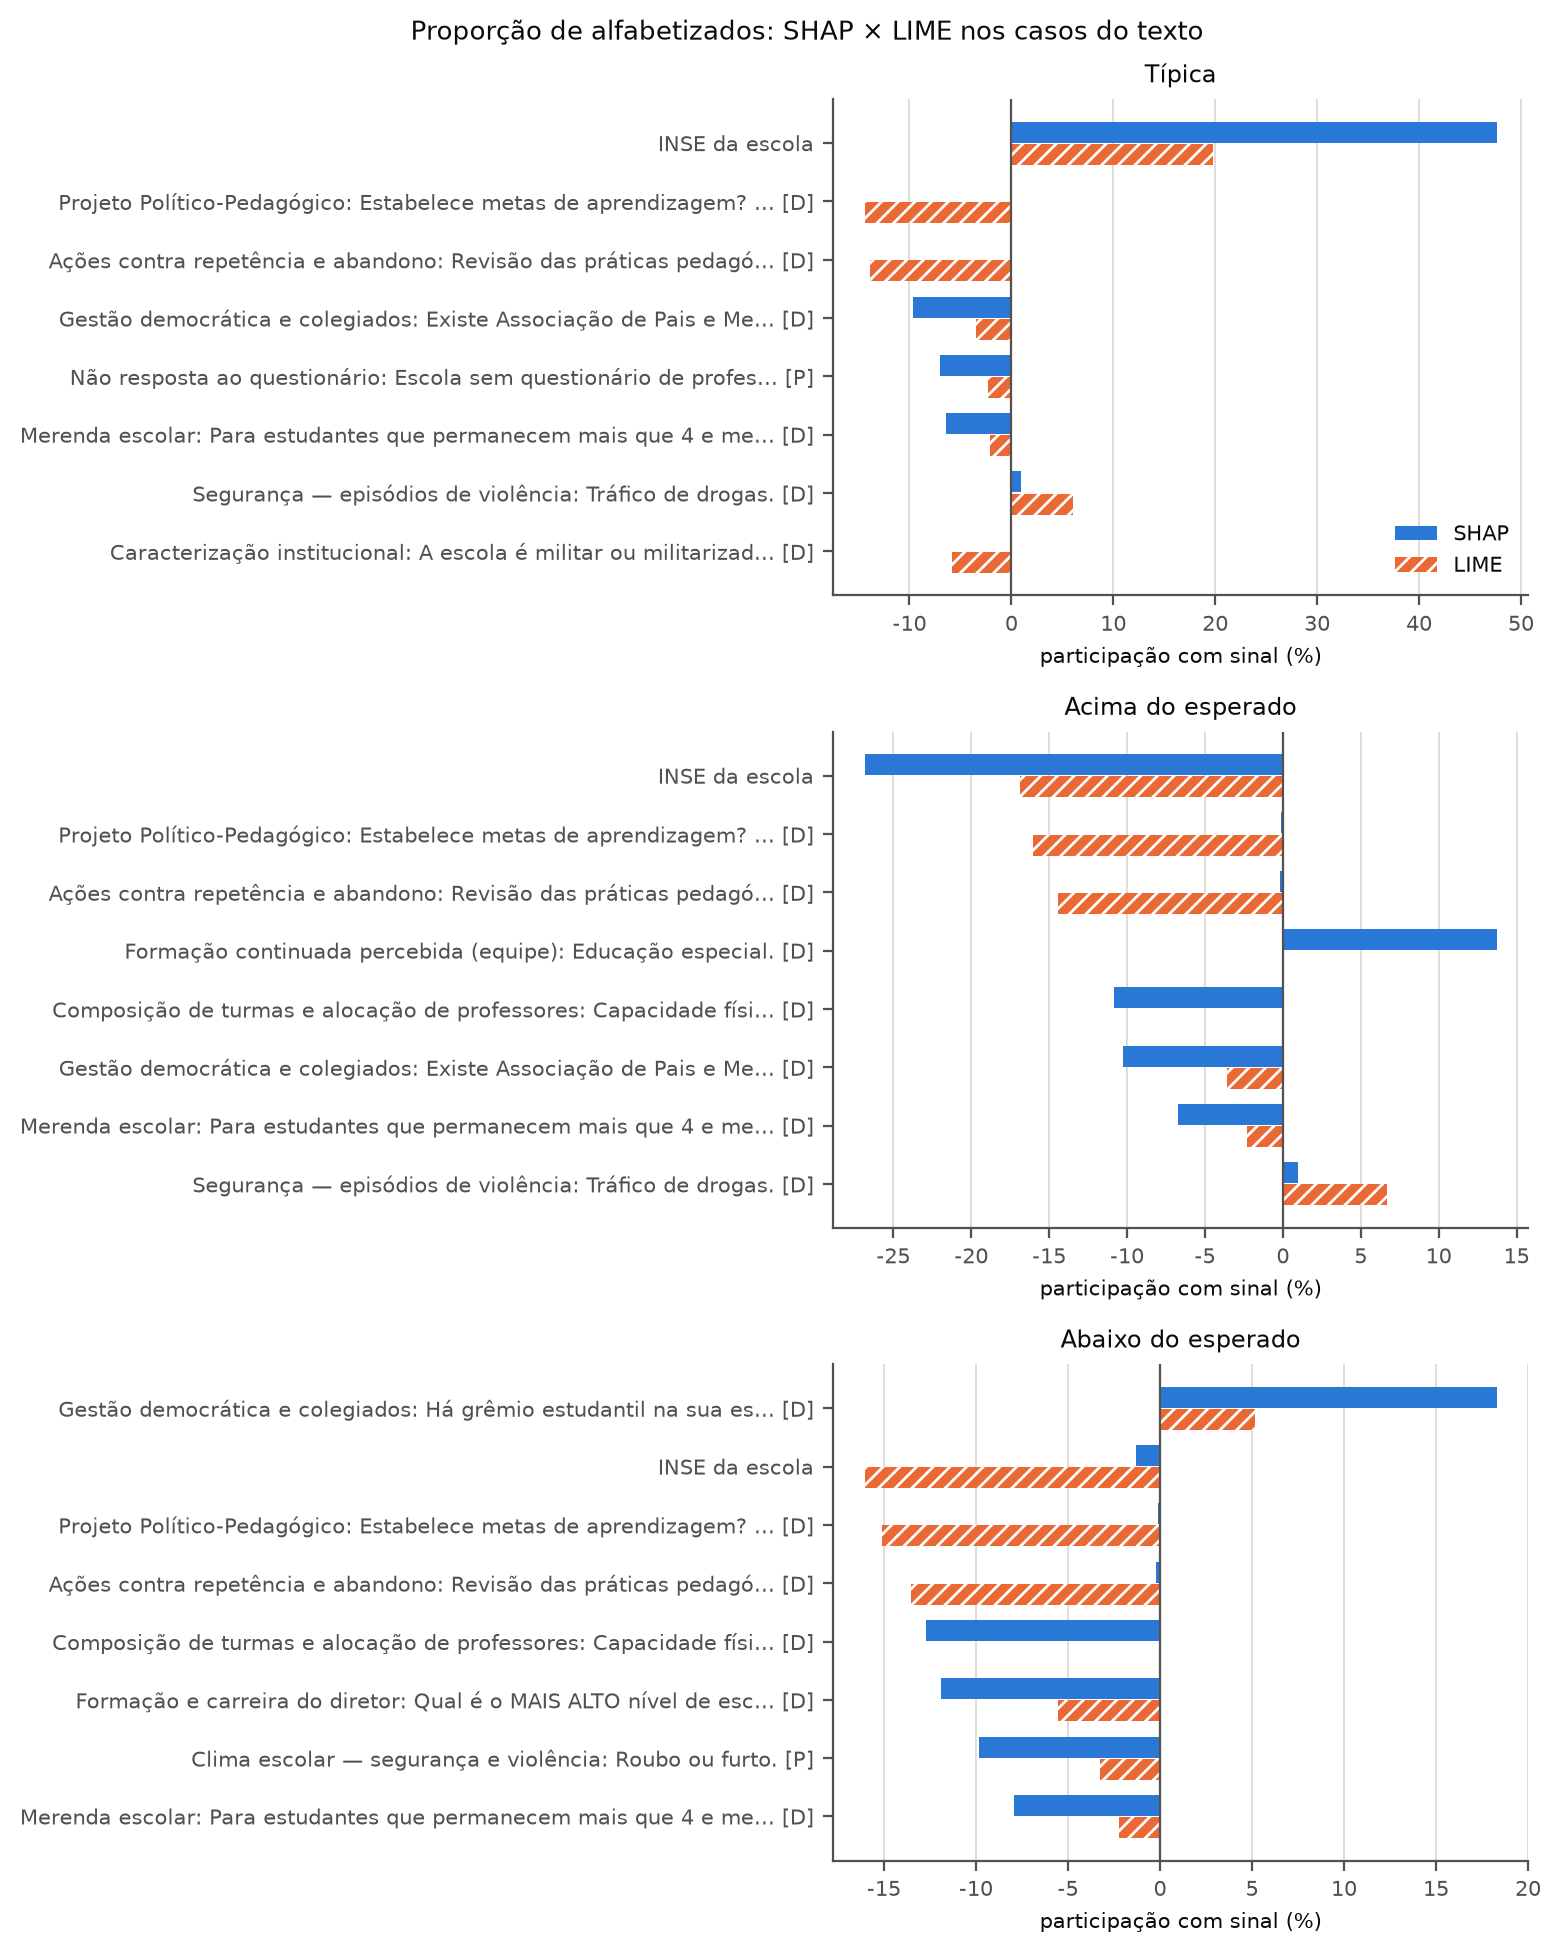
\includegraphics[width=\textwidth]{figuras/lime_shap_prop.png}
    \begin{flushleft}
    {\footnotesize Fonte: elaborada pelo autor, com base nos microdados do
    Saeb 2023 (Inep). Participação: contribuição da variável dividida pela
    soma das contribuições absolutas do método na escola.}
    \end{flushleft}
    \label{fig:ap-lime-shap-prop}
\end{figure}
